\documentclass{beamer}
\usepackage[utf8]{inputenc}
\usepackage{hyperref}
\usepackage{amsmath,amsfonts,amsthm,bm}
\usepackage{color}
\usepackage{minted}
\usepackage{graphicx} % Allows including images
\usepackage{booktabs} % Allows the use of \toprule, \midrule and \bottomrule in tables
\usepackage{tikz}
\usepackage{mhchem}
\usepackage{pgfplots}

\hypersetup{
    colorlinks=true,
    linkcolor=red,
    filecolor=magenta,      
    urlcolor=red,
}

\DeclareMathOperator*{\argmax}{argmax}
\DeclareMathOperator*{\argmin}{argmin}
\let \vec \mathbf

\mode<presentation> {
    \usetheme{CambridgeUS}
    %\setbeamertemplate{footline} % To remove the footer line in all slides uncomment this line
    \setbeamertemplate{footline}[page number] % To replace the footer line in all slides with a simple slide count uncomment this line
    \setbeamertemplate{navigation symbols}{} % To remove the navigation symbols from the bottom of all slides uncomment this line
}


\title[Extending Linear Methods]{Extending Linear Methods}

\author{Shyue Ping Ong}
\institute[UCSD]{University of California, San Diego\\
\medskip
}
\date{NANO281} % Date, can be changed to a custom date

\begin{document}


\begin{frame}
    \titlepage % Print the title page as the first slide
\end{frame}


\begin{frame}{Overview}
    \tableofcontents
\end{frame}


\section{Preliminaries}

\begin{frame}{Preliminaries}
    \begin{itemize}
        \item It is highly unlikely that the true function $f(X)$ is linear in $X$.
        \item In some cases, linearity is a reasonable assumption, e.g., a first order Taylor series expansion:
        \begin{equation*}
            f(x) = f(a) + f'(a) (x-a) + f''(a) \frac{(x-a)^2}{2!} + f'''(a) \frac{(x-a)^3}{3!} + ...
        \end{equation*}
        \item Examples where this is used in materials science - linear elasticity (Hooke's law), etc.
        \item More frequently, we perform a transformation of inputs to create a linear basis expansion.
    \end{itemize}
\end{frame}

\section{Transformation of inputs}

\begin{frame}{General concept}
    \begin{itemize}
        \item Express:
        \begin{equation*}
            f(X) = \sum_{m=1}^M \beta_m h_m(X)
        \end{equation*}
        where $h_m$ is the $m^{th}$ transformation of $X$.
        \item This is known as a linear basis expansion in $X$.
        \item The key lies in choice of the basis functions $h_m$.
    \end{itemize}
\end{frame}

\begin{frame}{Examples of basis expansions}
    \begin{itemize}
        \item $h_m(X) = X_j^2, h_m(X) = X_i X_j$
        \begin{itemize}
            \item Polynomial expansion to higher-order Taylor series terms.
            \item No. of terms increases exponentially with degree of polynomial. For $p$ variables, we have $O(p^2)$ square and cross-product terms in a quadratic model. For a degree $d$ polynomial, we have $O(p^d)$.
        \end{itemize}
        \item $h_m(X) = log(X_j), sqrt(X_j), exp(i X_j)$: non-linear transformations in $X$.
        \item $h_m(X) = I(L_m \leq X_k < U_m)$: Piece-wise division of regions of $X$. E.g., cubic splines.
        \item $h_m(X) = RBF(||X-X_m||)$: radial basis function, e.g., Gaussian. 
        \item Typically, basis functions are used simply to allow a more flexible representation of the data. The basis functions can span a very large (sometimes infinite) set, from which a selection has to be made:
        \begin{itemize}
            \item Restriction - Truncate the choice of basis functions using some criteria.
            \item Selection - Choose basis functions that contribute significantly to the fit.
            \item Regularization - Use the whole and/or very large subset and apply regularization techniques (e.g., ridge or LASSO) to restrict coefficients.
        \end{itemize}
    \end{itemize}
\end{frame}

\begin{frame}{Linearization from physical laws}
    \begin{itemize}
        \item Arrhenius law:
        \begin{equation*}
            r = A \exp(-\frac{E_a}{RT}) \longrightarrow log(r) = log(A) - \frac{E_a}{RT}
        \end{equation*}
        \item Ising model:
        \begin{equation*}
            H(\sigma) = - \sum_{<i, j>} J_{ij}\sigma_i \sigma_j - \mu \sum_j h_j \sigma_j
        \end{equation*}
        \begin{figure}
            \centering
            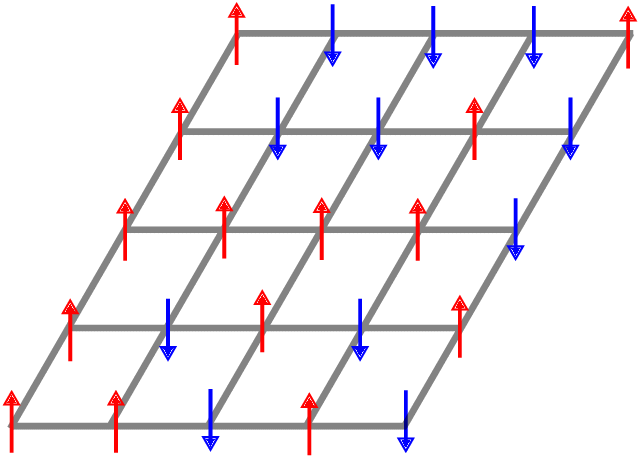
\includegraphics[width=0.3\textwidth]{figures/ising.png}
        \end{figure}
    \end{itemize}
\end{frame}


\begin{frame}{Compressive sensing for cluster expansions}
    \begin{itemize}
        \item Cluster expansion of energy on lattice points:
        \begin{equation*}
            H(\sigma) = E_0 + \sum_f J_f \prod_f(\sigma)
        \end{equation*}
        \item $\sigma$ is the vector representing occupation of lattice sites, $\prod_f$ are the cluster basis functions, $J_f$ are effective cluster interactions (ECIs).
        \item Compressive sensing: essentially a LASSO to solve for ECIs.\cite{nelsonCompressiveSensingParadigm2013}
        \begin{figure}
            \centering
            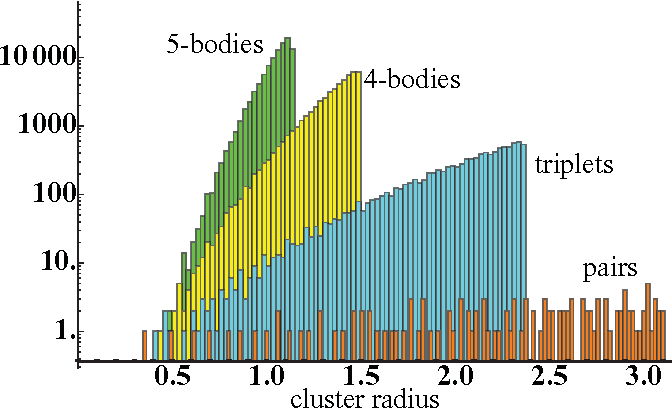
\includegraphics[width=0.4\textwidth]{figures/numberofclusters.png}
            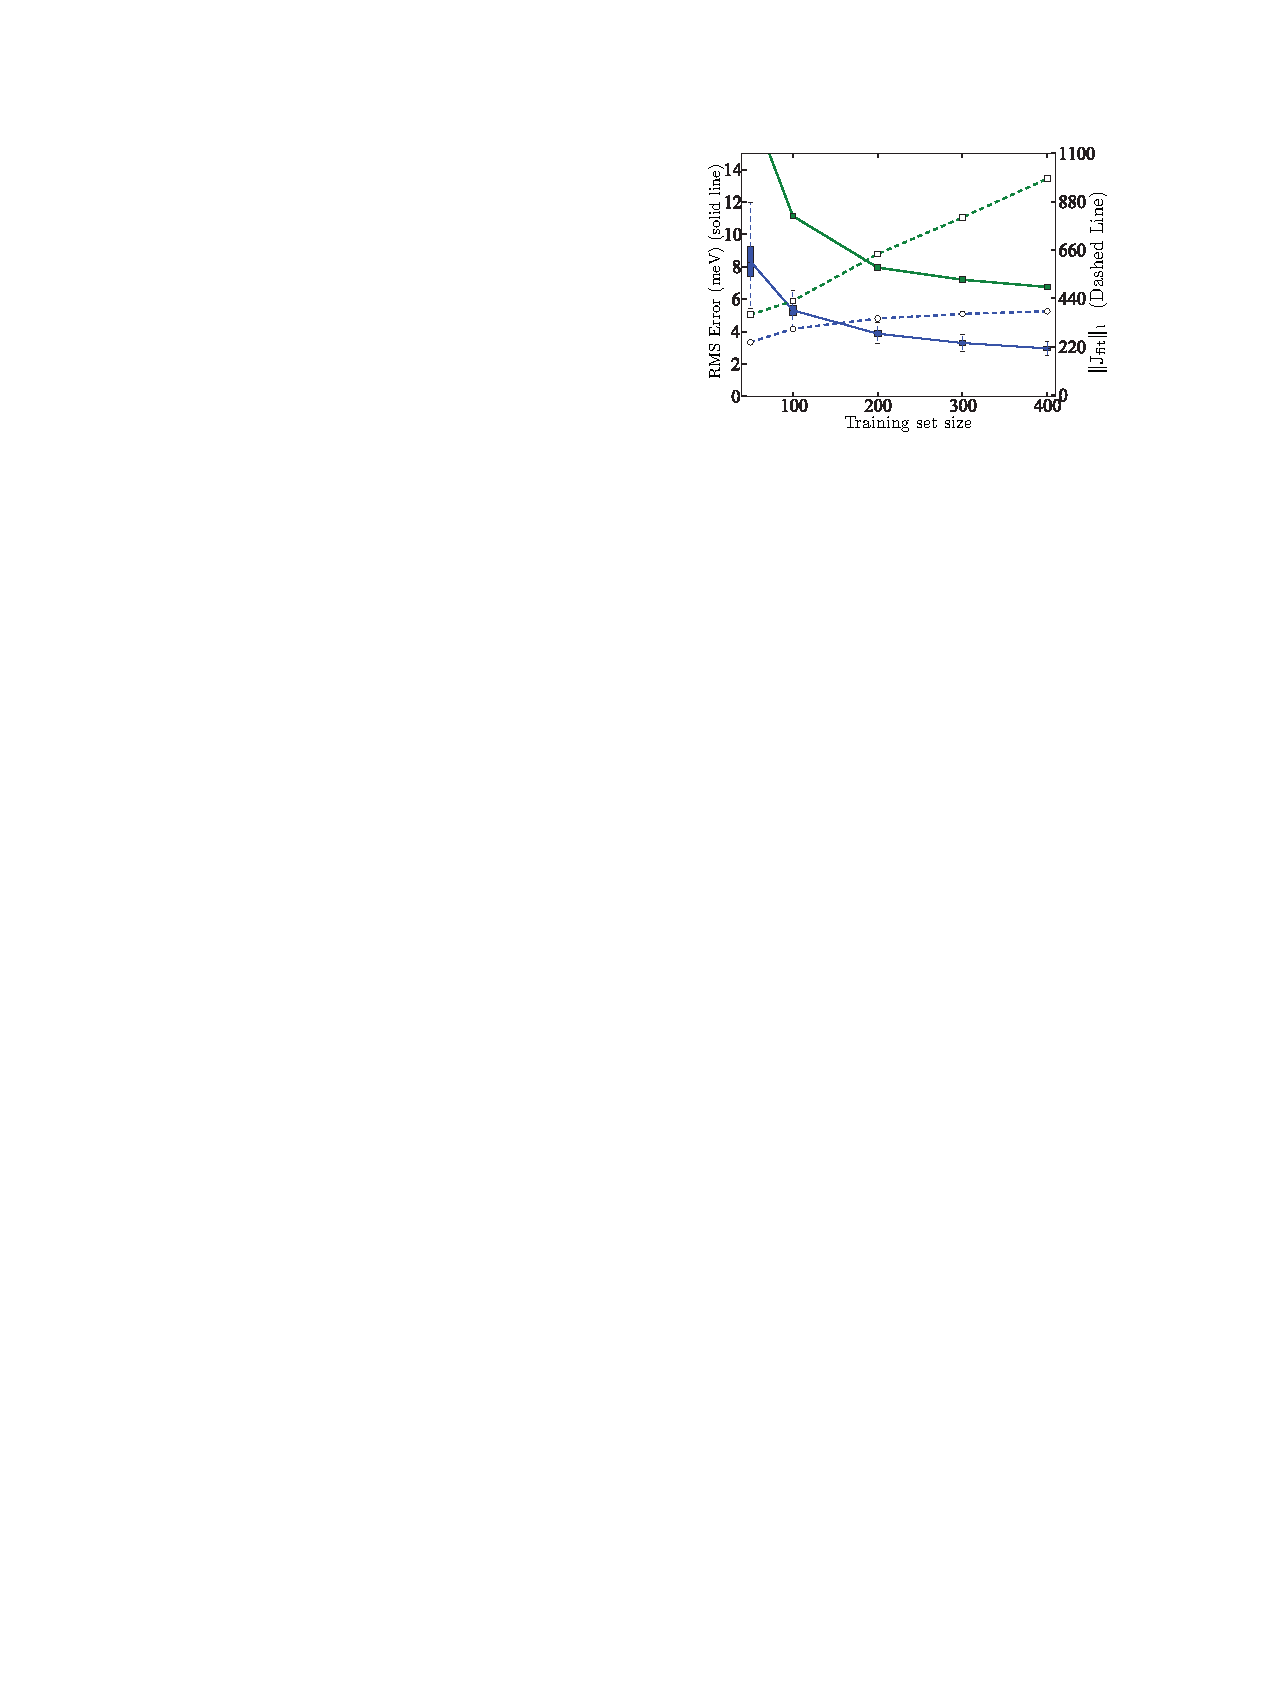
\includegraphics[width=0.4\textwidth]{figures/ecifit.pdf}
        \end{figure}
    \end{itemize}
\end{frame} 

\section{Piece-wise polynomials}

\begin{frame}{Piecewise polynomials}
    \begin{equation*}
        h_1(X) = I(X < \xi_1), h_2(X) = I(\xi_1 \leq X < \xi_2), h_3(X) = I(X \geq \xi_2)
    \end{equation*}
    \begin{columns}
    \column{0.5\textwidth}
    \begin{figure}
        \centering
        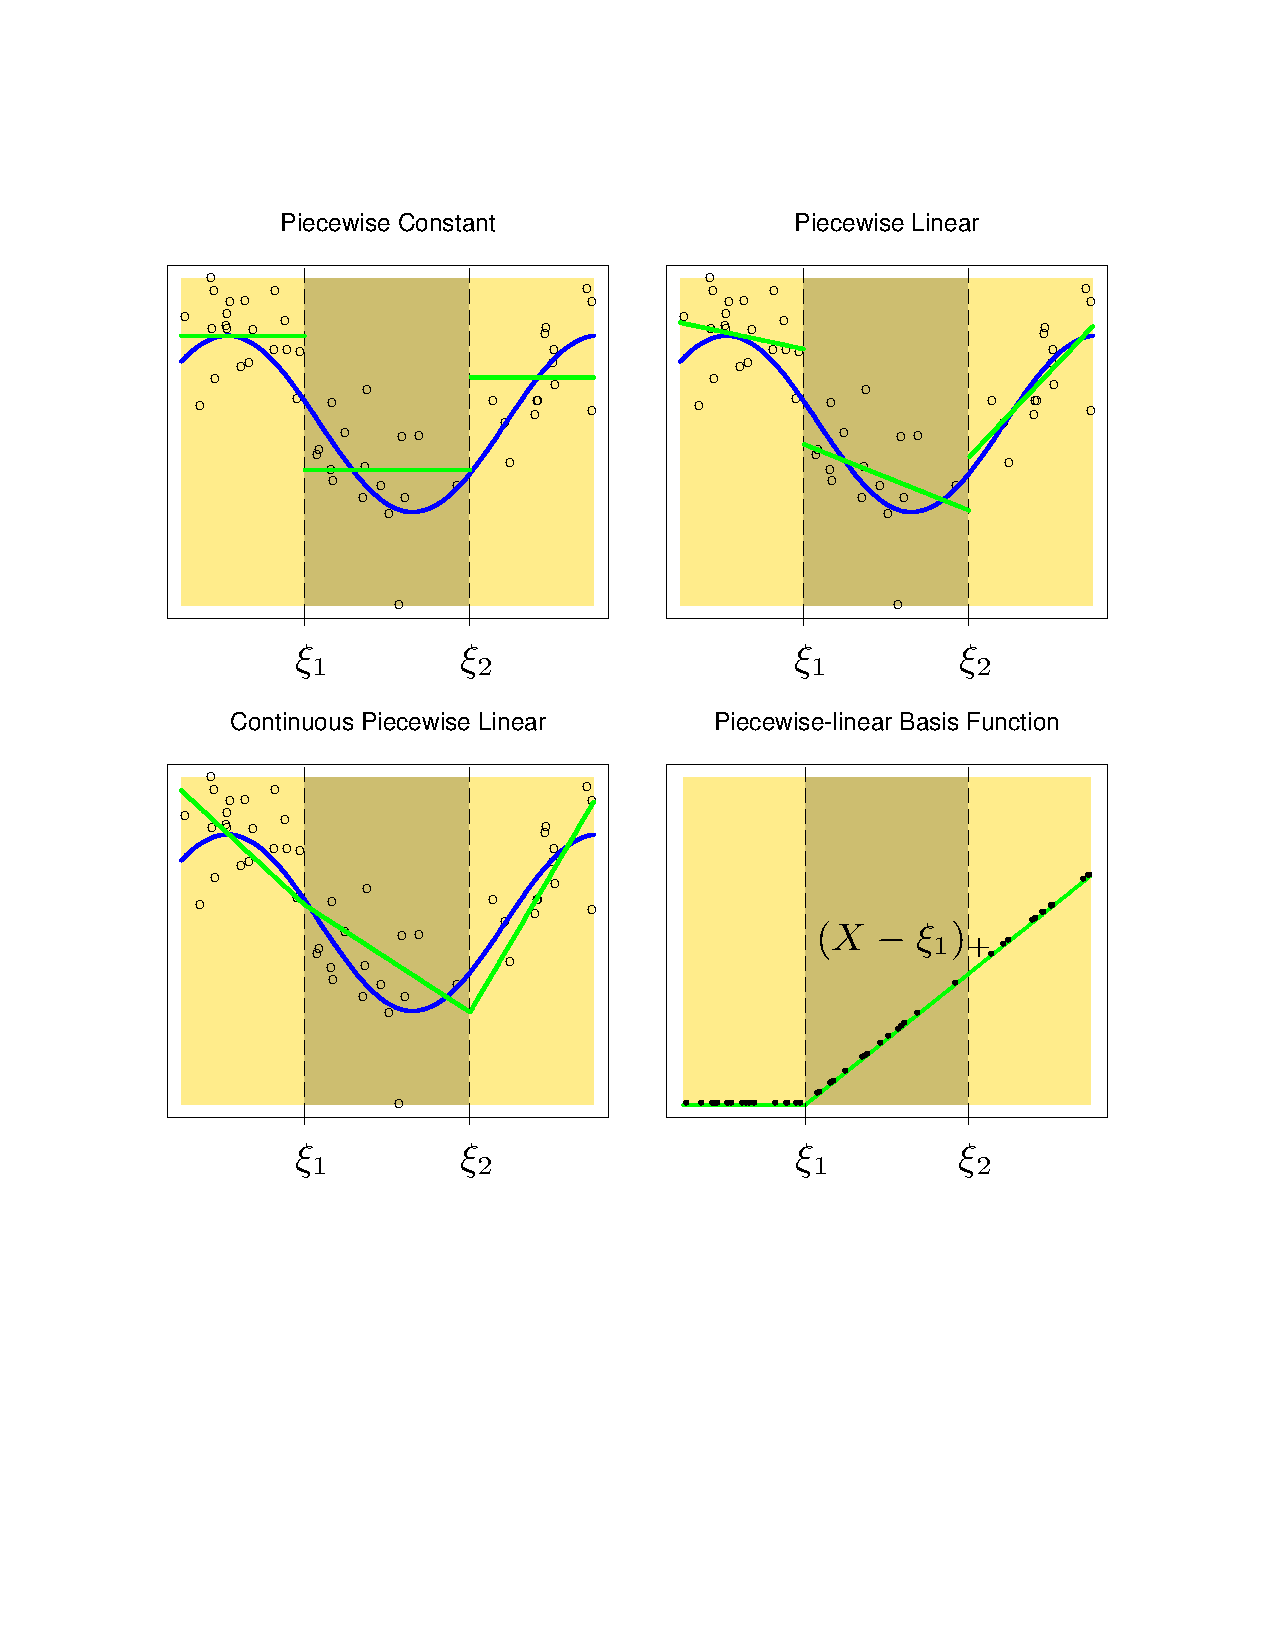
\includegraphics[width=0.8\textwidth]{figures/piecewisefits.pdf}
    \end{figure}
    \column{0.5\textwidth}
    Parameters:
    \begin{itemize}
        \item No. of knots
        \item Order of polynomial
        \item Continuity at knots (value, first derivative, second derivative, etc.). For a polynomial of order $N$, we usually want all derivatives $< N$ to be continuous. 
    \end{itemize}
    \end{columns}
\end{frame} 


\begin{frame}{Cubic splines}
    \begin{columns}
    \column{0.5\textwidth}
    \begin{figure}
        \centering
        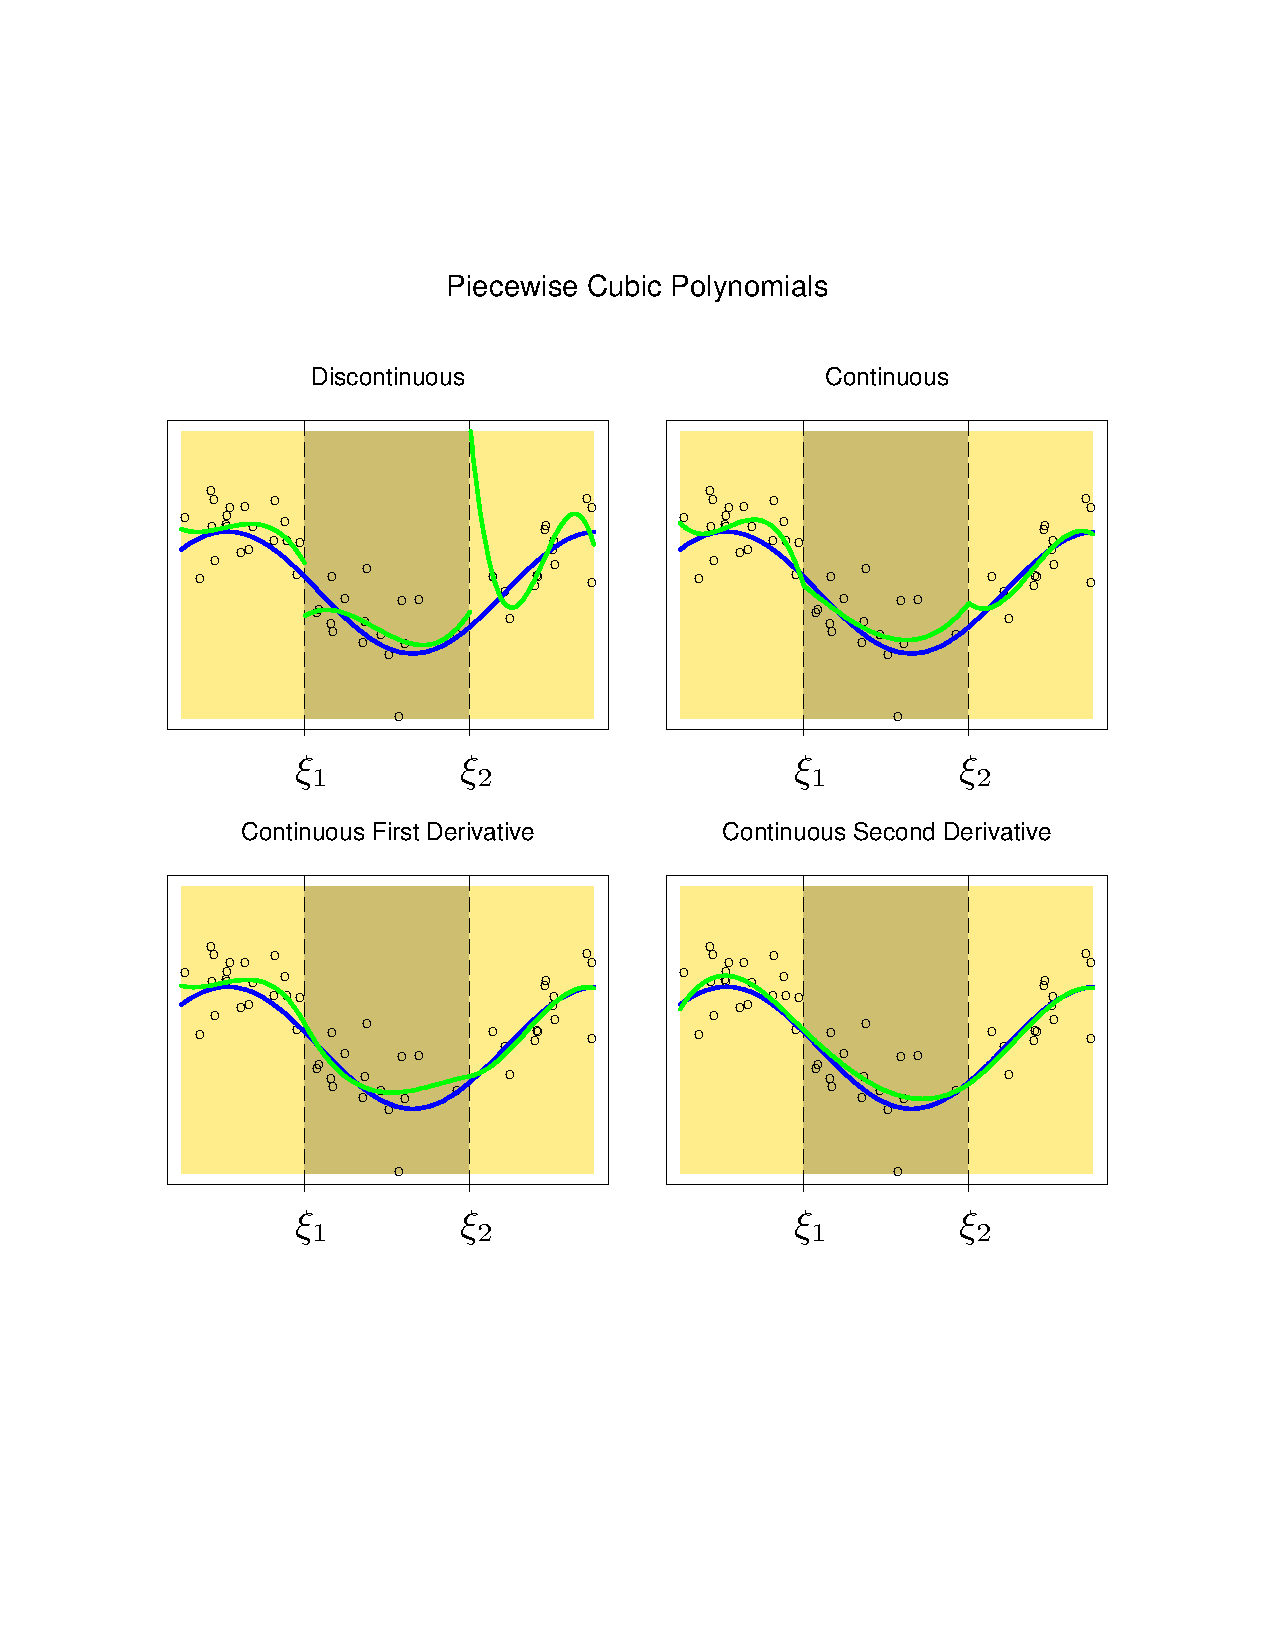
\includegraphics[width=0.8\textwidth]{figures/piecewisecubic.pdf}
    \end{figure}
    \column{0.5\textwidth}
    \begin{itemize}
        \item Probably the most commonly used.
        \item Continuous 1st and 2nd derivatives.
        \item Natural cubic spline: polynomial is linear beyond boundaries.
        \item Smoothing spline: Use  regularization to control complexity:
        \begin{eqnarray*}
            RSS(f, \lambda) = \sum_{i=1}^N \{y_i - f(x_i)\} ^ 2 \\
            + \lambda \int \{f''(t)\}^2 dt
        \end{eqnarray*}
    \end{itemize}
    \end{columns}
\end{frame}


\begin{frame}{Examples of cubic spline fitting}
    \begin{itemize}
        \item Spline-based Modified Embedded Atom Method (MEAM)
        \begin{eqnarray*}
            E = \sum_{i <j} \phi(r_{ij}) + \sum_i U(n_i), \\
            n_i = \sum_j \rho(r_{ij}) + \sum_{i < k, j,k!=i} f(r_{ij}) f(r_{ik})g[cos(\theta_{jik})]
        \end{eqnarray*}
        where $\phi$, $U$, $\rho$, $f$ and $g$ can be approximated by cubic splines. 
        \begin{figure}
            \centering
            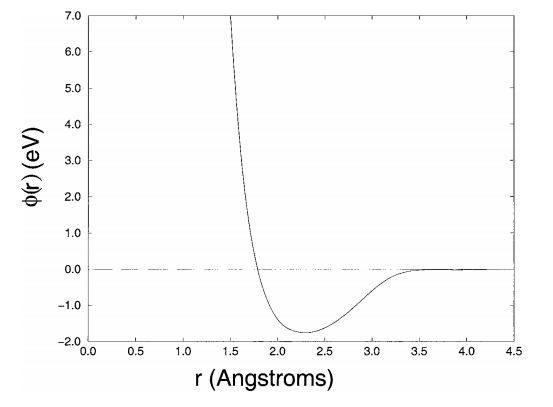
\includegraphics[width=0.45\textwidth]{figures/meam-phi.png}
            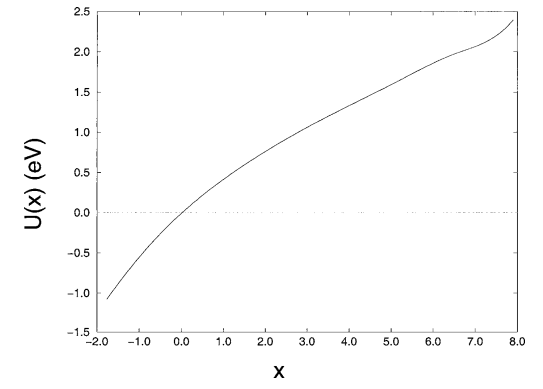
\includegraphics[width=0.45\textwidth]{figures/meam-u.png}

        \end{figure}
    \end{itemize}
\end{frame} 


\begin{frame}[fragile]{Demo: Cubic spline fitting in scipy}
    \begin{minted}{python}
import numpy as np
## Import CubicSpline from scipy
from scipy.interpolate import CubicSpline

## x, y data for generating the spline fitting
x = np.arange(10)
y = np.sin(x)

## Fit the spline
cs = CubicSpline(x, y)

## Generate new x values
xs = np.arange(-0.5, 9.6, 0.1)

## Perform the interpolation on the new points
ys = cs(xs)
\end{minted}
\end{frame} 


\section{Gaussian basis functions}


\begin{frame}{Gaussian basis functions}
    \begin{equation*}
        h_m(x) = \exp(-k(x - x_m) ^ 2)
    \end{equation*}
    \begin{itemize}
        \item Gaussian functions centered at $x_m$.
        \item Other similar types of functions include Lorentzian ($h_m(x) = \frac{1}{1 + kx^2}$), Gaussian-Lorentzian, Voigtian, Pearson type IV, and beta profiles.
    \end{itemize}
\end{frame} 


\begin{frame}{Example: Rietveld refinement}
\begin{figure}
    \centering
    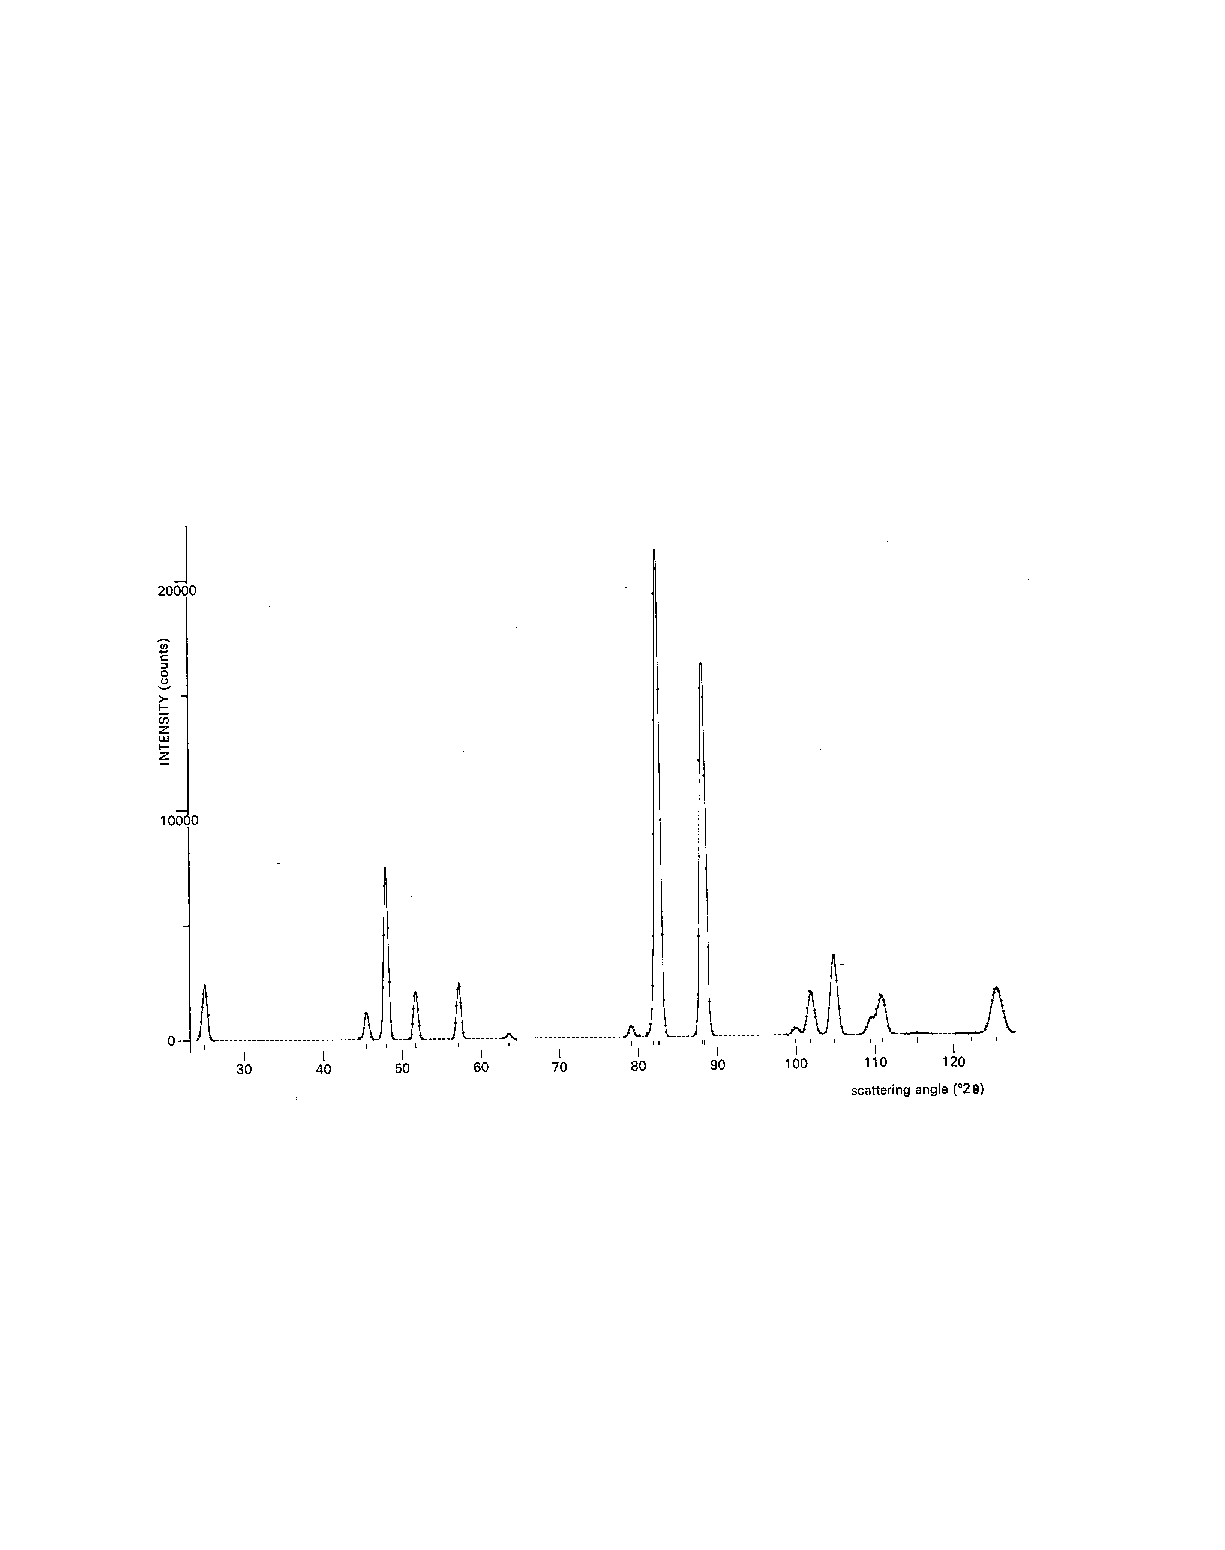
\includegraphics[width=0.5\textwidth]{figures/rietveld.pdf}
    \caption{Neutron powder diffraction diagram of \ce{CaUO4}}
\end{figure}
    \begin{itemize}
        \item Least squares fitting of theoretical line profile to match a measured diffraction pattern (e.g., X-ray, neutron).\cite{rietveldProfileRefinementMethod1969}
    \end{itemize}
\end{frame} 


\begin{frame}{Example: Rietveld refinement, contd.}
    \begin{itemize}
        \item Peak shape function:
        \begin{equation*}
            PSF(\theta) = \Omega(\theta) \otimes \Lambda(\theta) \otimes \Psi(\theta) + b(\theta)
        \end{equation*}
        \item $\Omega$: Instrument broadening, $\Lambda$: Wavelength dispersion, $\Psi$: Specimen function.
        \item For single phase, minimize:
        \begin{equation*}
            \Phi = \sum_{i=1}^N w_i \left ( Y_i^{obs} - \left ( b_i + K \sum_{j=1}^m I_jy_j(x_j)\right )\right )^2
        \end{equation*}
        \item where $y_j(x_j)$ is typically a pseudo-Voigt (mix of Gaussian and Lorentizan function) function.
        \item Note that the background ($b_i$) holds no useful structural information and should be minimized in experiments.
    \end{itemize}
\end{frame} 



\section{Wavelet and Fourier basis functions}


\begin{frame}
\frametitle{Wavelet smoothing}
\begin{columns}
\column{0.5\textwidth}
\begin{figure}
    \centering
    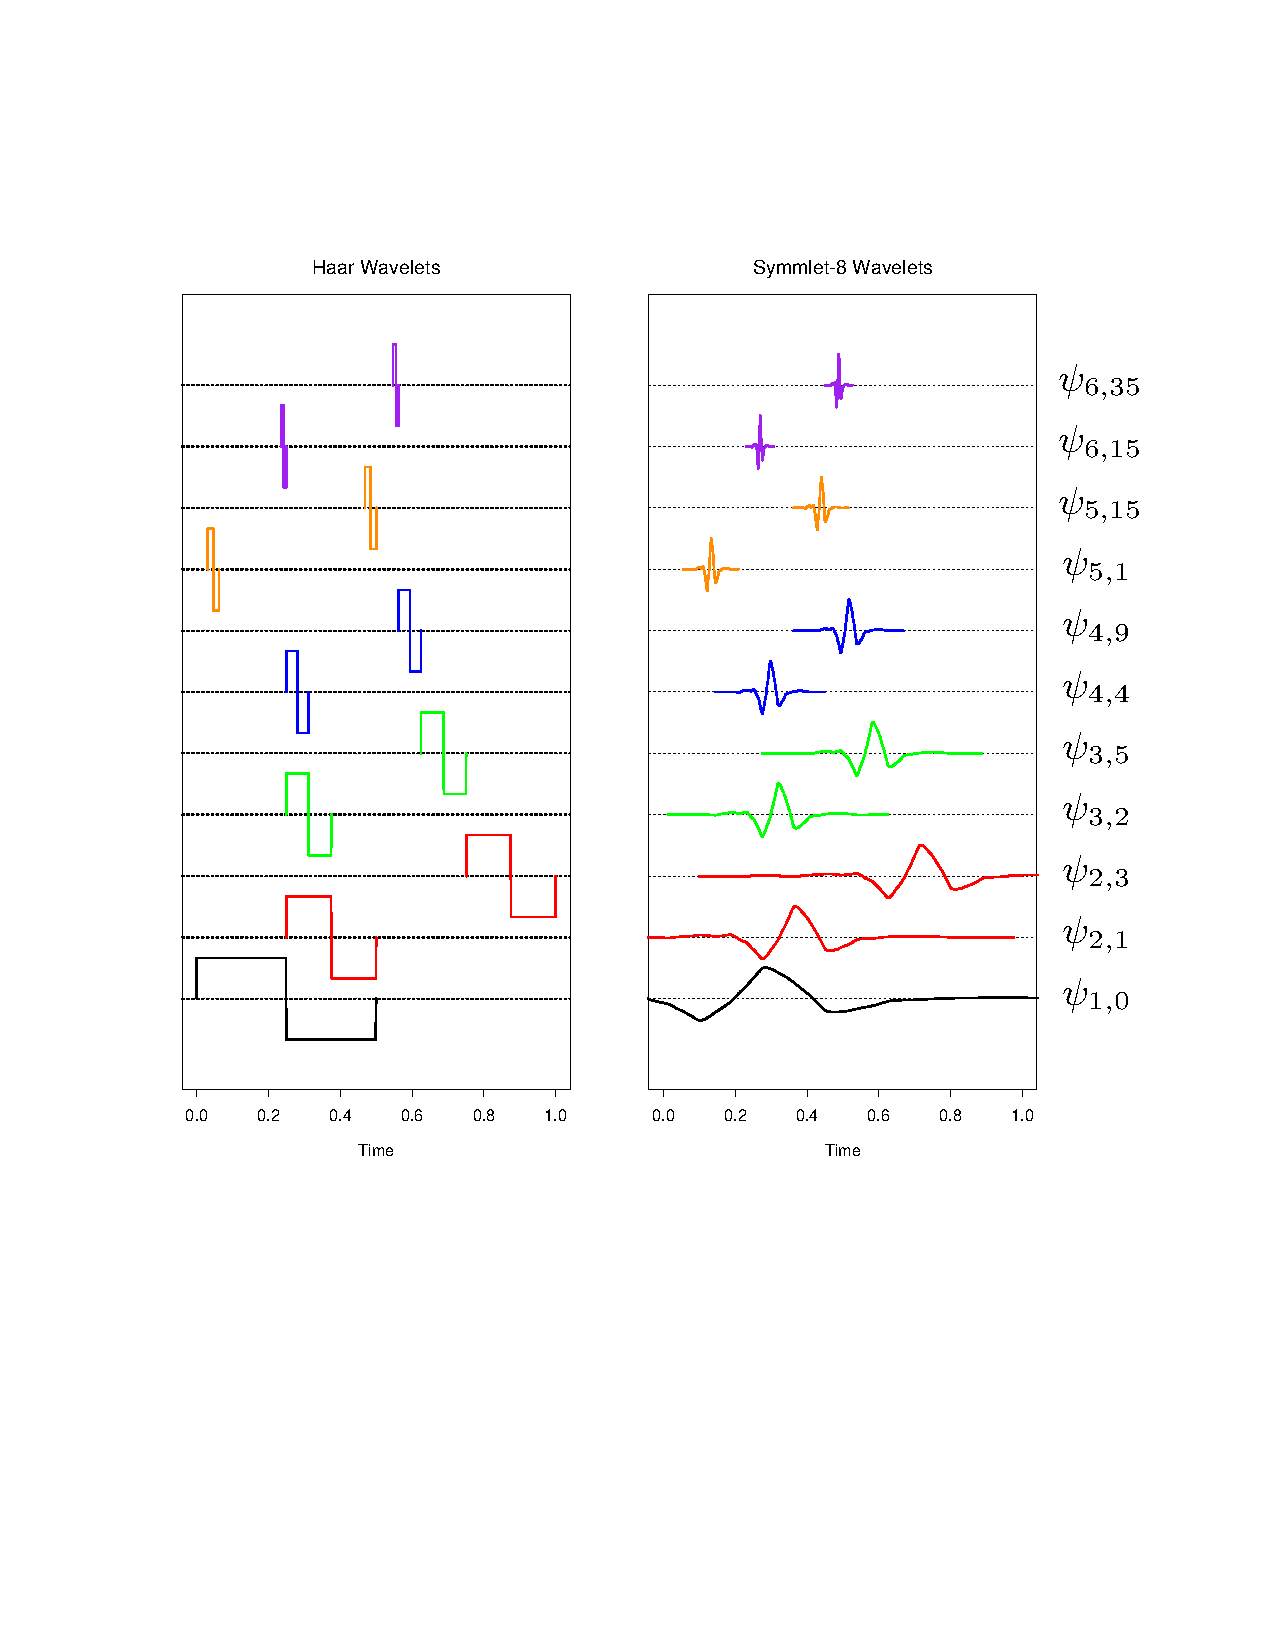
\includegraphics[width=\textwidth]{figures/wavelets.pdf}
\end{figure}
\column{0.5\textwidth}
    \begin{itemize}
        \item Complete orthonormal basis
        \item Shrink and select toward \textbf{sparse} representation.
        \item Able to represent both time and frequency localization efficiently (Fourier basis can only do frequency localization).
    \end{itemize}
\end{columns}
\end{frame} 


\begin{frame}{Example: NMR Spectroscopy}
\begin{columns}
\column{0.5\textwidth}
\begin{figure}
    \centering
    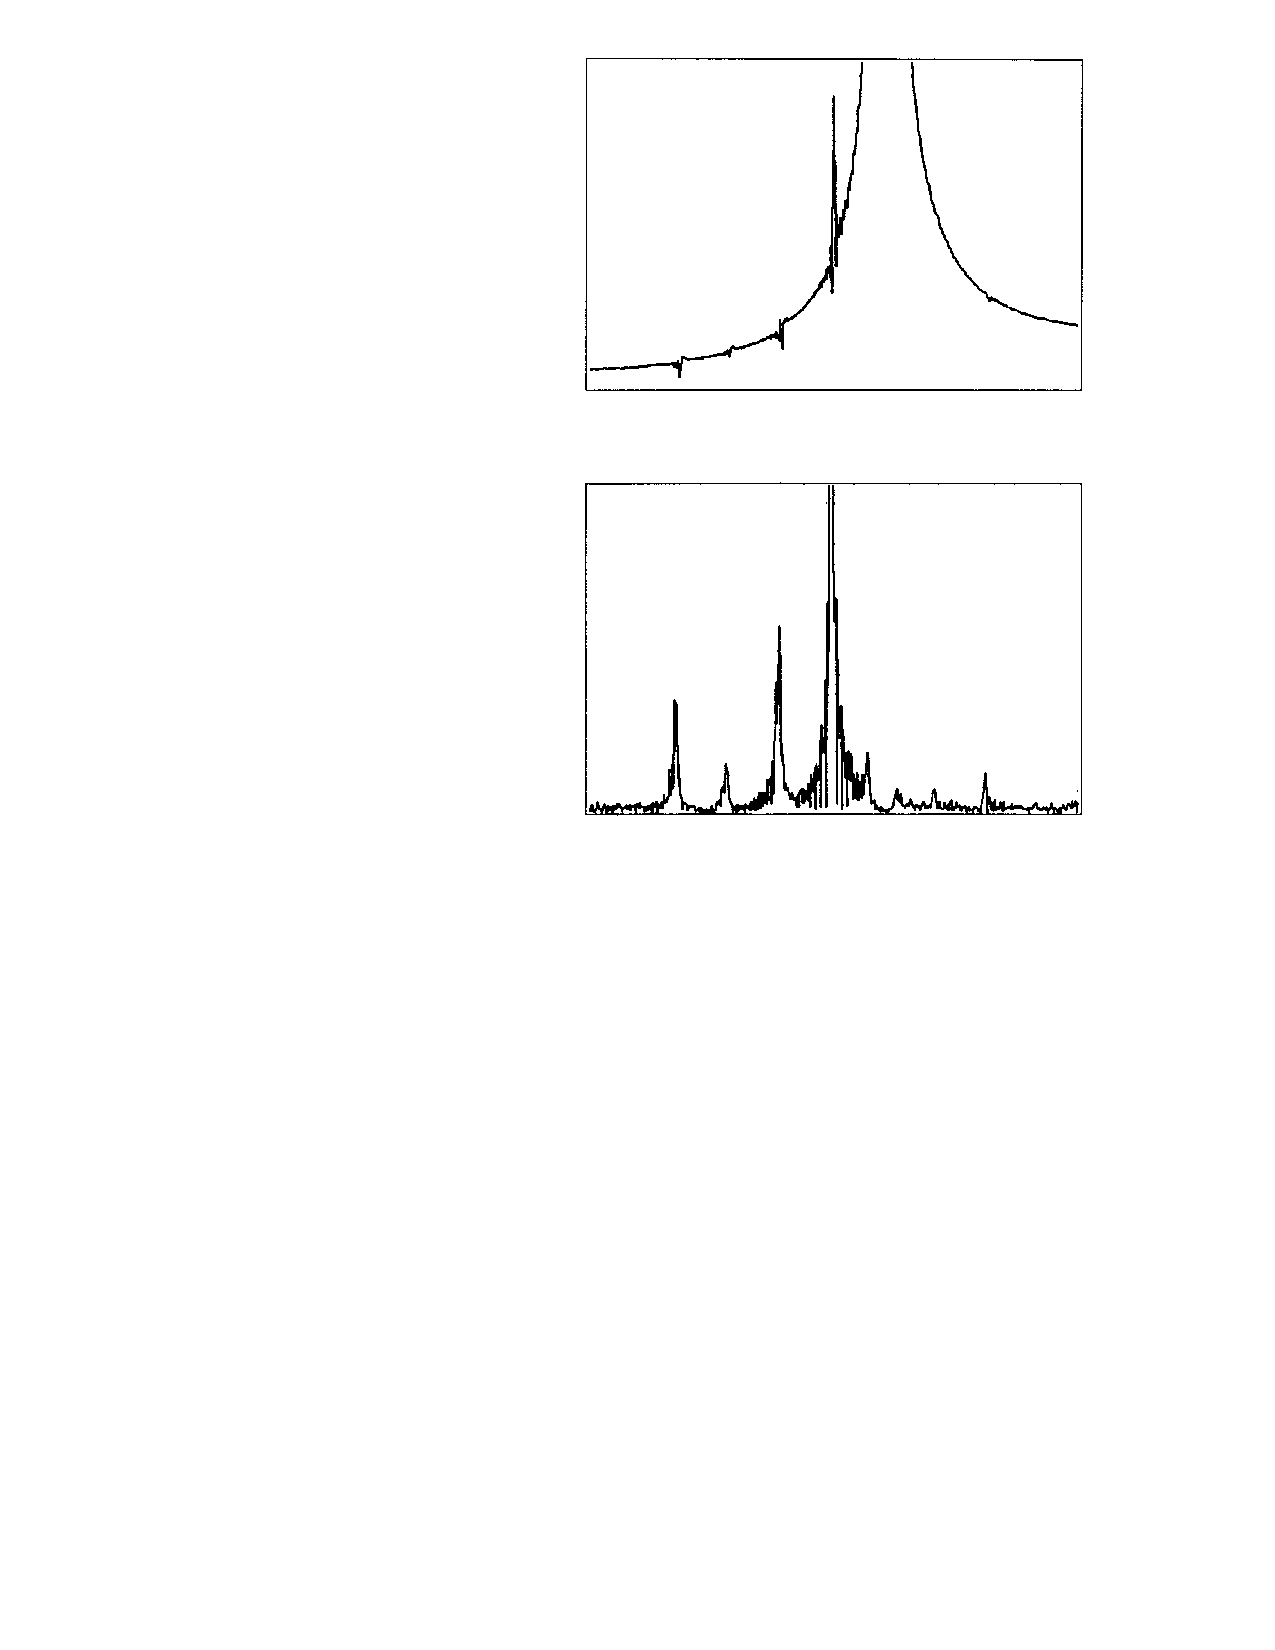
\includegraphics[width=0.6\textwidth]{figures/nmrwavelet.pdf}
    \caption{Subtraction of a large spectral line: (top) the original spectrum of polyethylene, (bottom) reconstructed spectrum after removal of \ce{CH2} peak.\cite{baracheContinuousWaveletTransform1997}}
\end{figure}
\column{0.5\textwidth}
    Applications:
    \begin{itemize}
        \item Suppression of large unwanted spectral line (left).
        \item Rephasing spectrum perturbed by time-dependent magnetic field.
        \item Noise filtering
        \item Detecting phases in a mixture
    \end{itemize}
\end{columns}
\end{frame} 

\begin{frame}{Example: Fourier transform for analysis of extended X-ray absorption fine structure (EXAFS)}
    
    \begin{columns}
    \column{0.5\textwidth}
    \begin{figure}
        \centering
    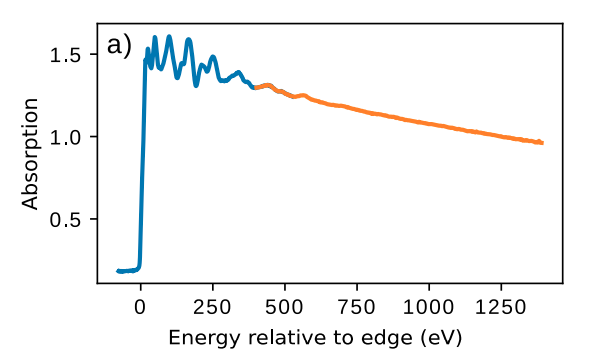
\includegraphics[width=0.6\textwidth]{figures/EXAFS-1.png}
    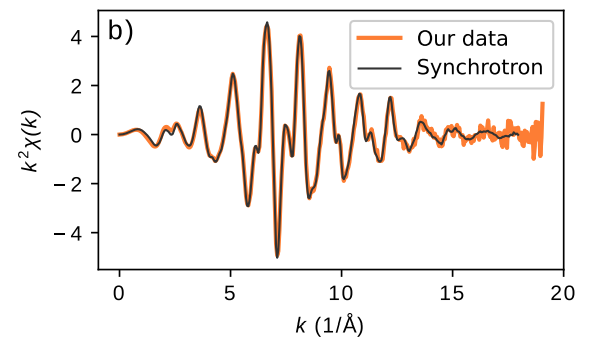
\includegraphics[width=0.6\textwidth]{figures/EXAFS-2.png}
    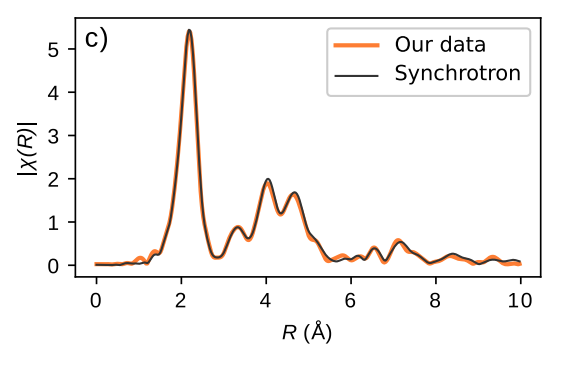
\includegraphics[width=0.6\textwidth]{figures/EXAFS-3.png}
    \end{figure}
    \column{0.5\textwidth}
    \begin{itemize}
        \item (a) The extended edge (orange part) contains information of atom chemical environment.
        \item (b) Subtract the background, convert energy to k-space unit, and multiply the normalized intensity by $k^2$
        \item (c) Fourier transform $k$-space information to real space and obtain the first shell bond length. 
    \end{itemize}
    \end{columns}
    
\end{frame} 

\begin{frame}{Bibliography}
    \bibliographystyle{unsrt}
    \bibliography{refs}
\end{frame}


\begin{frame}
    \Huge{\centerline{The End}}
\end{frame}

\end{document}

